\documentclass[12pt]{article}

% Dimensiones exactas para YouTube (1280x720 px)
\usepackage[paperwidth=1280pt, paperheight=720pt, margin=0pt]{geometry}
\usepackage[dvipsnames]{xcolor}
\usepackage{graphicx}
\usepackage{fontspec}
\usepackage{tikz}

% --- CONFIGURACIÓN DE FUENTE ---
% Asegúrate de tener Inter instalada en Ubuntu (sudo apt install fonts-inter)
\setmainfont{Inter}[BoldFont=* Bold]

% --- VARIABLES DEL RETO ---
\newcommand{\numeroReto}{8º}
\newcommand{\tituloSerie}{reto de demostración con Lean 4}
\newcommand{\descripcionReto}{Una sucesión que posee infinitos términos
  con valor absoluto superior a 10 no puede converger a un límite cuyo
  valor absoluto sea menor que 5.}

% Espaciado de palabras: 1.5em para que se lean bien a distancia
\newcommand{\espacioPalabras}{
    \spaceskip=0.25em \relax
}

\definecolor{leanblue}{HTML}{007ACC}

\begin{document}
\pagestyle{empty}
\noindent
\begin{tikzpicture}[x=1pt, y=1pt, inner sep=0pt, outer sep=0pt]

    % Fondo blanco
    \fill[leanblue] (0,0) rectangle (1280,720);

    % --- 1. TÍTULO (ARRIBA) ---
    % Subimos un poco el título para dejar espacio al logo gigante
    % Mantenemos la franja azul característica
    \node[anchor=north, text width=1250pt, align=center] at (640, 705) {
        {\fontsize{54pt}{75pt}\selectfont \espacioPalabras \bfseries \color{white} \numeroReto\ \tituloSerie}
    };

    % --- 2. LOGO (CENTRO - OCUPANDO TODO EL ANCHO) ---
    % Al poner width=1280pt y quitar la restricción de height,
    % el logo llegará de borde a borde. keepaspectratio evita que se deforme.
    % Línea de acento naranja/ocre
    \fill[Orange!90!black] (0, 210) rectangle (1280, 222);
    \node[anchor=center] at (640, 415) {
        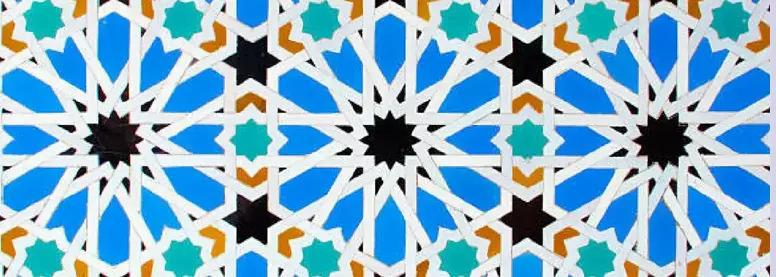
\includegraphics[width=1280pt, keepaspectratio]{logo.jpeg}
    };

    % --- 3. DESCRIPCIÓN (ABAJO) ---
    % Mantenemos la franja azul característica
    \fill[leanblue] (0, 0) rectangle (1280, 210);
    % Línea de acento naranja/ocre
    \fill[Orange!90!black] (0, 210) rectangle (1280, 222);

    \node[anchor=center, text width=1250pt, align=center] at (640, 105) {
        {\fontsize{54pt}{75pt}\selectfont \espacioPalabras \bfseries \color{white} \descripcionReto}
    };

\end{tikzpicture}
\end{document}

%%% Local Variables:
%%% mode: LaTeX
%%% TeX-master: t
%%% End:
